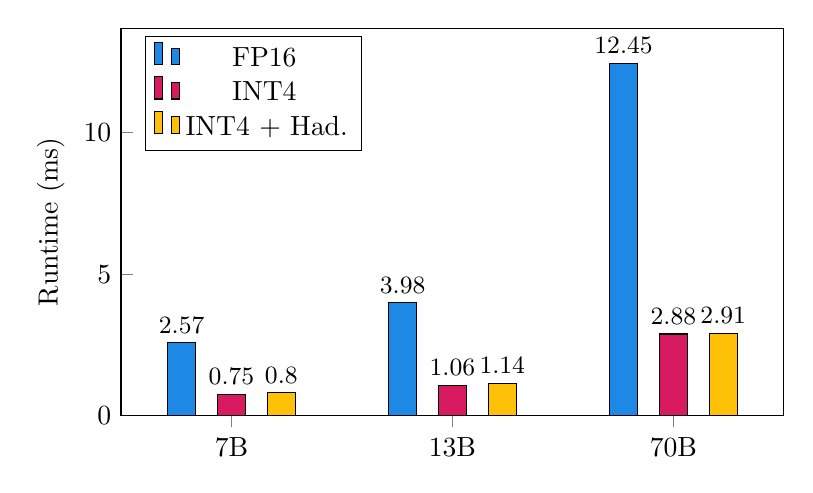
\begin{tikzpicture}  
\definecolor{col1}{HTML}{1E88E5}
\definecolor{col2}{HTML}{D81B60}
\definecolor{col3}{HTML}{FFC107}

\begin{axis}[
    width=10cm, 
    height=6.5cm,  
    ybar=8pt,  
    enlarge x limits=0.25,  
    legend style={at={(0.2,0.98)},  
      anchor=north},  
    ylabel={Runtime (ms)},
    symbolic x coords={7B, 13B, 70B},  
    xtick=data,  
    nodes near coords,  
    nodes near coords align={vertical},  
    nodes near coords style={font=\small},
    ymin = 0,
    ytick pos=left,
    xtick pos=left,
    ]  
\addplot[fill=col1] coordinates {(7B, 2.569) (13B,3.983)  (70B, 12.45)};
\addplot[fill=col2] coordinates {(7B,0.749) (13B,1.063) (70B,2.881)}; 
\addplot[fill=col3] coordinates {(7B,0.798) (13B,1.142) (70B,2.911)}; 
\legend{FP16\,, INT4\,, INT4 + Had.}  
\end{axis}  
\end{tikzpicture}  
  

